%%%%%%%%%%%%%% COPYRIGHT INFORMATION %%%%%%%%%%%%%%
% Template by
% Author: Sascha Frank 
% Nov. 2006
% University Freiburg 
% www.informatik.uni-freiburg.de/~frank/
% Distributed freely for non-commercial use

%%%%%%%%%%%%%%%%%%%%% PREAMBLE %%%%%%%%%%%%%%%%%%%%%
\documentclass{beamer}
\usepackage{beamerthemeshadow}
\usepackage{lmodern}
\usepackage{pifont}
\usepackage{color}

% to draw graphs
\usepackage {tikz}
\usetikzlibrary{positioning}
\definecolor{processblue}{cmyk}{0.96,0,0,0}

% include frame number on each frame
\setbeamertemplate{footline}{\quad \insertframenumber/\inserttotalframenumber}
\newcommand{\cmark}{\ding{51}} % check-mark
\newcommand{\xmark}{\ding{55}} % X-mark
\newcommand{\inv}{^{-1}}
\newcommand{\e}{\varepsilon}
\newcommand{\E}{\mathbb{E}}
\newcommand{\N}{\mathbb{N}}
\renewcommand{\P}{\mathbb{P}}
\newcommand{\R}{\mathbb{R}}
\newcommand{\Var}{\mathbb{V}}
\newcommand{\X}{\mathcal{X}}
\newcommand{\Y}{\mathcal{Y}}
\newcommand{\Z}{\mathcal{Z}}
\newcommand{\dist}{\operatorname{dist}}
\newcommand{\vi}{{\vec i}}

%%%%%%%%%%%%%%%%%%%%% DOCUMENT %%%%%%%%%%%%%%%%%%%%%
\begin{document}
\title{Inferring Functional Connectivity in fMRI data}
\author[Singh]{Shashank Singh \\
Advisors: Barnab\'as P\'oczos, Timothy Verstynen
}
\institute{36-757 ADA I}
\date{February 25, 2014}
\frame{\titlepage}

\frame{\frametitle{Outline}
\begin{enumerate}
\item {\color{red} Data \uncover<2->{- multiple views}}
\item Goals
\item Methods
\end{enumerate}
}

\section{The Data}
\subsection{Local Brain Activity View}
\frame{\frametitle{Local Brain Activity View}
\begin{figure}[h!]
  \centering
  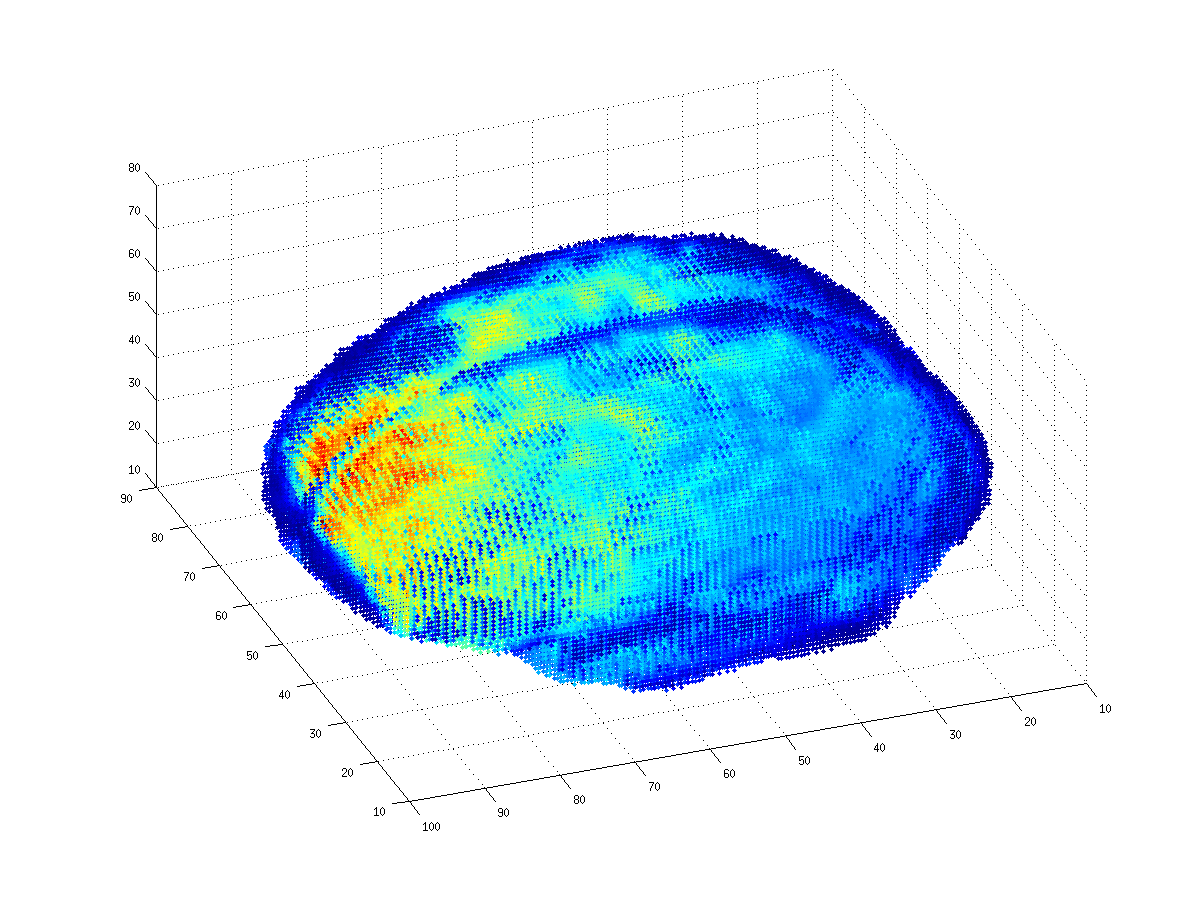
\includegraphics[width=0.6\linewidth]{eda1}
  \label{fig:mirror_fig}
\end{figure}
\vspace{-5mm}
Each time frame is a snapshot of $V \approx 1.6 \times 10^5$ voxel activities.
}

\subsection{Time Series View}
\frame{\frametitle{Time Series View}
\begin{figure}[h!]
  \centering
  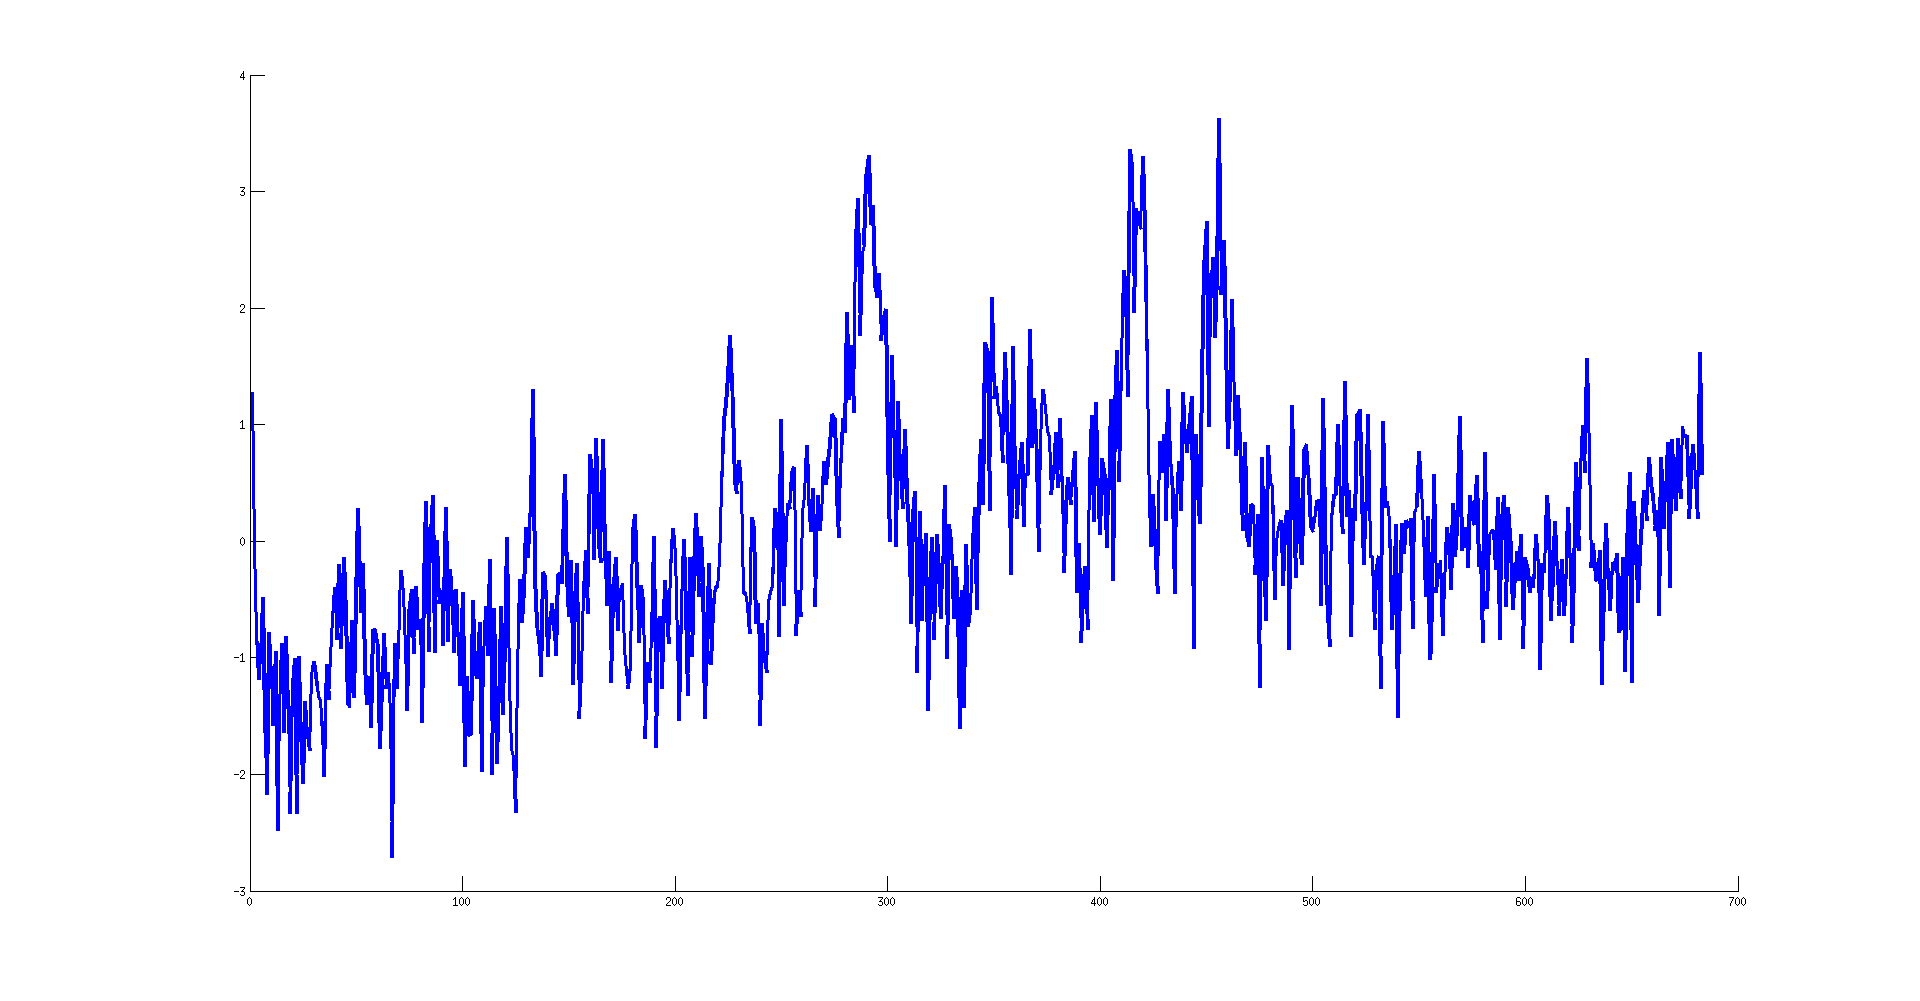
\includegraphics[width=0.6\linewidth]{voxel1_over_time}
  \label{fig:mirror_fig}
\end{figure}
\vspace{-5mm}
Each voxel is $683$ point time series.
}

\subsection{Brain Parcellation}
\frame{\frametitle{Brain Parcellation}
\begin{figure}[h!]
  \centering
  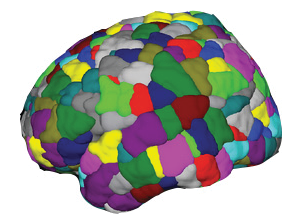
\includegraphics[width=0.5\linewidth]{parcellated_brain}
  \label{fig:mirror_fig}
\end{figure}
\vspace{-5mm}
\begin{center}
Parcellate to reduce dimension ($R = 600$).
\end{center}
}

\section{Goals}
\frame{\frametitle{Outline}
\begin{enumerate}
\item Data
\item {\color{red} Goals}
\item Methods
\end{enumerate}
}

\frame{\frametitle{Higher-Order Connectivity and Information Flow}
Want to test for (conditional) dependence between voxels
\begin{figure}[h]
\centering
\begin{tikzpicture}[-latex, auto, node distance=4 cm and 5cm, on grid,
semithick, state/.style={circle, top color=white, bottom color=processblue!20,
draw, processblue, text=blue, minimum width=1 cm}]
  % seed
  \node[state] (n0) at (1,5) {Seed};
  % layer 1
  \node[state] (n11) at (2.8, 3.4)  {};
  \node[state] (n15) at (2.8, 6.6)  {};
  % layer 2
  \node[state] (n23) at (4.6, 6)    {};
  \node[state] (n25) at (4.6, 7.2)  {};
  % layer 3
  \node[state] (n33) at (6.4, 3.4)  {};
  \node[state] (n35) at (6.4, 6.6)  {};
  % layer 4
  \node[state] (n43) at (8.2, 5)    {};

\foreach \from/\to in {n0/n15,n0/n11,n33/n0,n15/n25,n15/n23,n25/n35,n23/n35,n11/n33,n33/n43,n35/n43}
    \draw (\from) -- (\to);
\end{tikzpicture}
\end{figure}
}

\frame{\frametitle{Goals}
\begin{itemize}
\item Want to evaluate methods for inferring functional connectivity
\begin{itemize}
\item ``whole-brain'' (high-dimensional) context
\item account for vascular anatomy
\item Want to distinguish higher-order (indirect) connectivity
\end{itemize}
\end{itemize}
}

\section{Methods}
\frame{\frametitle{Outline}
\begin{enumerate}
\item Data
\item Goals
\item {\color{red} Methods}
\end{enumerate}
}

\frame{\frametitle{Statistical Methods}
\begin{enumerate}
\item Time Series Methods
\begin{itemize}
\item Granger Causality/Transfer Entropy
\end{itemize}
\pause
\item Sparse Prediction Methods
\begin{itemize}
\item Lasso/Elastic Net, FuSSO
\end{itemize}
\pause
\item Graphical Model Learning Methods
\begin{itemize}
\item Chow-Liu/PC algorithms with novel independence tests
\end{itemize}
\end{enumerate}
}

\frame{\frametitle{\null}
\begin{center}
{\LARGE Thanks!} \\
\vspace{10mm}
Questions?
\end{center}
}

\end{document}
